\chapter{Evaluation}
\label{chap:evaluation}

We are going to compare the new or changed components of our system with the old ones.
We will not discuss the soundness of the components, because these are covered by unit tests and tests comparing results between our implementation and the reference implementations.

\section{Proof of Retrievability Verification}

The trivial verification method is to download the whole file and compare it against the original.
This defeats the point of distributed storage, but it can be optimized by comparing the hash of the file instead of the file itself.
This method requires too much bandwidth ($O(N)$) and is therefore slow,
but it is a 100\% accurate and requires only $O(N)$ computation (where $N$ is the size of the file) on the client side and $O(1)$ space for the hash.

Can we do better?
We can precompute multiple hashes from the file concatenated with a random string (salt) and store these hashes together with the salts.
Then, we for each verification we can send the salt, then the storage node sends back the hash of the file with the salt, and finally we compare the hash to the one we have precomputed.
This method requires $O(1)$ bandwidth and $O(N)$ computation on the client side (the cost of precomputing each hash) and $O(1)$ space for the hashes and salts.

Keeping the bandwidth low is important, because it is the slowest part of the verification process.
The computation can be usually parallelized and make use of data locality to be much faster than network communication.
This is where our current implementation lies.
The Proof of Retrievability protocol we use requires $O(N^3)$ matrix multiplication algorithm reducible to $O(N^{2.37287})$ \cite{matrixmultiplication} for matrix multiplication during the precomputation step.
Since the matrices we are multiplying are of size $O(\sqrt{N})$, the total cost of the precomputation step is $O(N^{3/2})$.
Also, the matrices are special, so in reality we end up with close to $O(N)$ time.
The verification step requires $O(N)$ server computation and $O(\sqrt{N})$ client computation, as well as $O(\sqrt{N})$ bandwidth.
The space requirement is $O(N)$ for the server and $O(\sqrt{N})$ for the client.
These numbers can be further improved with a better Proof of Retrievability protocol \cite{pormerkle}.
This is marginally better thanks to the lower bandwidth and storage required on the client.
We would like to argue that these are the two most important resources because of the goals of the client - they want to store their data in the system, i.e., they want to use as little space as possible, and they want to be able to audit their data as fast as possible, i.e., they want to use as little bandwidth as possible.
It does not make sense to compare algorithms with different CPU and bandwidth requirements because the network communication can either be really fast or really slow, depending on the network conditions, distance between peers, etc.
Therefore, we will only present results for the time required to initialize a file and audit it on a local machine to give an idea of the performance of the system.

\begin{table}
  \myfloatalign
  \pgfplotstabletypeset[
    col sep=comma,
    header=true,
    string type,
    every head row/.style={%Define the top and mid lines
      before row=\toprule,
      after row=\midrule
    },
    every last row/.style={%Define the bottom line
      after row=\bottomrule
    },
    columns={Operation, Naive, Current implementation},
    columns/Operation/.style={column name=Operation, column type={>{\bfseries}r|}},
    columns/Naive/.style={column name=Naive, column type={c|}},
    columns/Current implementation/.style={column type={c}},
  ]{
    Operation, Naive, Current implementation
    {Init client cost}, $O(N)$, $O(N^{3/2})$
    {Init server cost}, $O(N)$, $O(N)$
    {Init bandwidth}, $O(N)$, $O(N)$
    {Audit client cost}, $O(N)$, $O(\sqrt{N})$
    {Audit server cost}, $O(N)$, $O(N)$
    {Audit bandwidth}, $O(1)$, $O(\sqrt{N})$
    {Storage server}, $O(N)$, $O(\sqrt{N})$
    {Storage client}, $O(1)$, $O(\sqrt{N})$

  }
  \caption[]{Theoretical comparison of the naive optimized (old implementation) and the Proof of Retrievability (current implementation)}
  \label{tab:pretty-table}
\end{table}

\begin{figure}
  \myfloatalign
  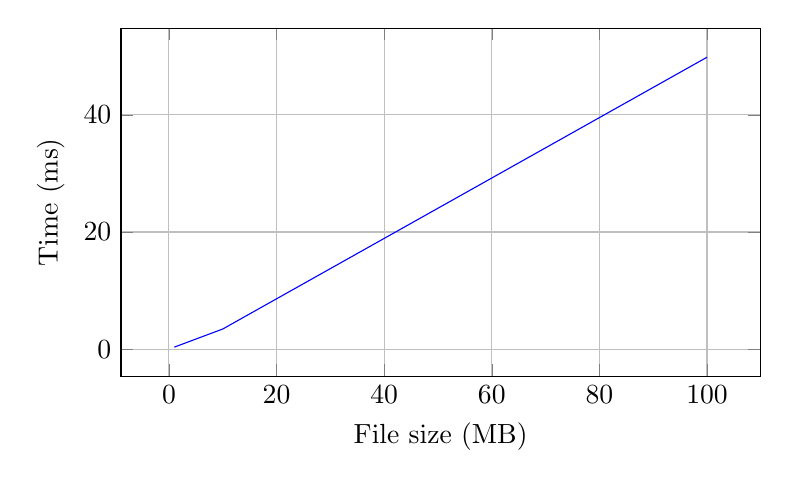
\begin{tikzpicture}
    \begin{axis}[
      xlabel={File size (MB)},
      ylabel={Time (ms)},
      grid=major,
      width=0.8\textwidth,
      height=6cm,
    ]
    \addplot[mark=., blue] coordinates {
      (1, 0.347597)
      (10, 3.439716)
      (100, 49.84325)
    };
    \end{axis}
  \end{tikzpicture}
  \caption[]{Time required to initialize a file. Larger tests (up to 1gb files) have been excluded from the graph because they are hard to visualize, but they exhibit the same linear trend.}
  \label{fig:pretty-graph}
\end{figure}

\begin{figure}
  \myfloatalign
  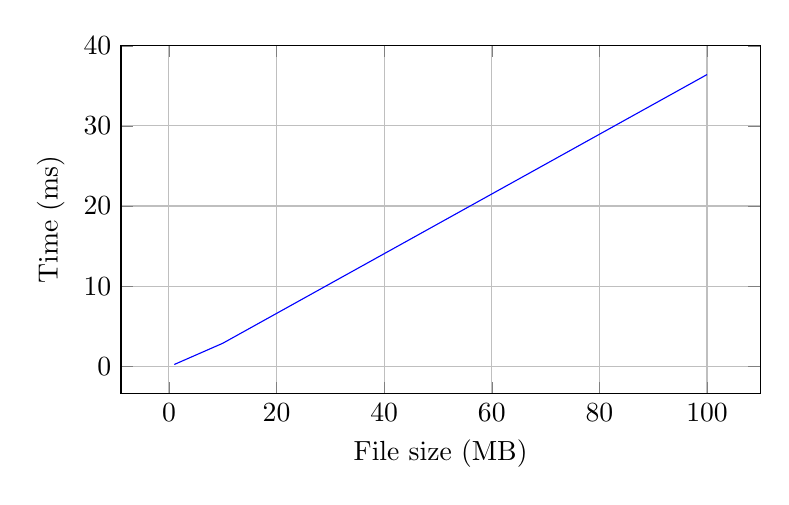
\begin{tikzpicture}
    \begin{axis}[
      xlabel={File size (MB)},
      ylabel={Time (ms)},
      grid=major,
      width=0.8\textwidth,
      height=6cm,
    ]
    \addplot[mark=., blue] coordinates {
      (1, 0.221211)
      (10, 2.867223)
      (100, 36.410966)
    };
    \end{axis}
  \end{tikzpicture}
  \caption[]{Time required to audit a file on the Verifier and the Keeper.}
  \label{fig:pretty-graph}
\end{figure}

\begin{figure}
  \myfloatalign
  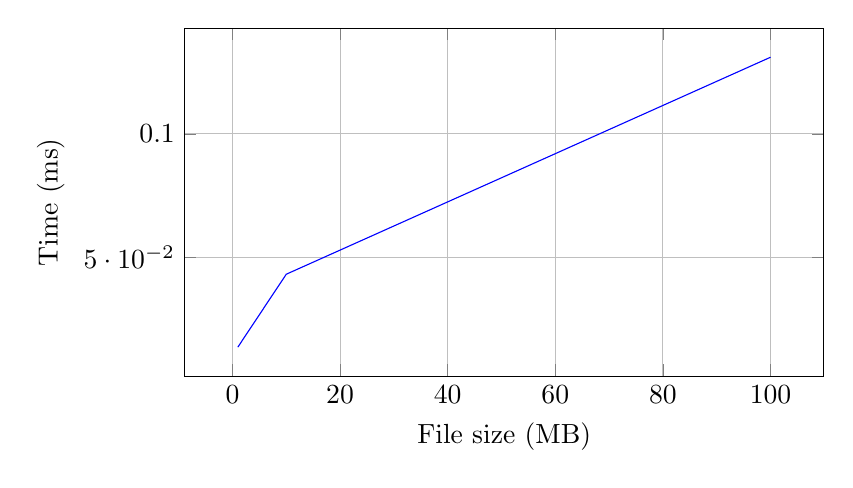
\begin{tikzpicture}
    \begin{axis}[
      xlabel={File size (MB)},
      ylabel={Time (ms)},
      grid=major,
      width=0.8\textwidth,
      height=6cm,
    ]
    \addplot[mark=., blue] coordinates {
      (1, 0.013607)
      (10, 0.043147)
      (100, 0.131054)
    };
    \end{axis}
  \end{tikzpicture}
  \caption[]{Time required to audit a file from the Verifier's perspective only.}
  \label{fig:pretty-graph}
\end{figure}

The conclusion from this is that the current implementation has some milliseconds (less than 1 second for 1 GB files) preprocessing overhead, but this allows much faster auditing.
The audit is comparable to the init time because they essentially do the same computation.
However, if we exclude the server time, the audit time is a magnitude faster than the init time.
This achieved our goal of putting as little load on the Verifier (client) as possible.
The results also confirm our theoretical time complexity analysis.

\section{Cryptographic puzzle}

We use a cryptographic puzzle to prevent Sybil attacks by limiting how fast a node can join the network.
The puzzle is a proof of work, i.e., a computation that is easy to verify but hard to compute.
We are using Sha3-256 \cite{sha3} as the hash function, and we require the hash to start with a certain number of zeros.
The number of zeros is a parameter of the system, and it can be changed to adjust the difficulty of the puzzle.
Having 4 leading zeros requires about 1.5 seconds on a modern CPU, and it is a good tradeoff between security and usability.
Each added zero makes the puzzle on average 20 times harder.
This means we can start the system off with 4 leading zeros and then increase the number of leading zeros if needed as the network grows.

\begin{figure}
  \myfloatalign
  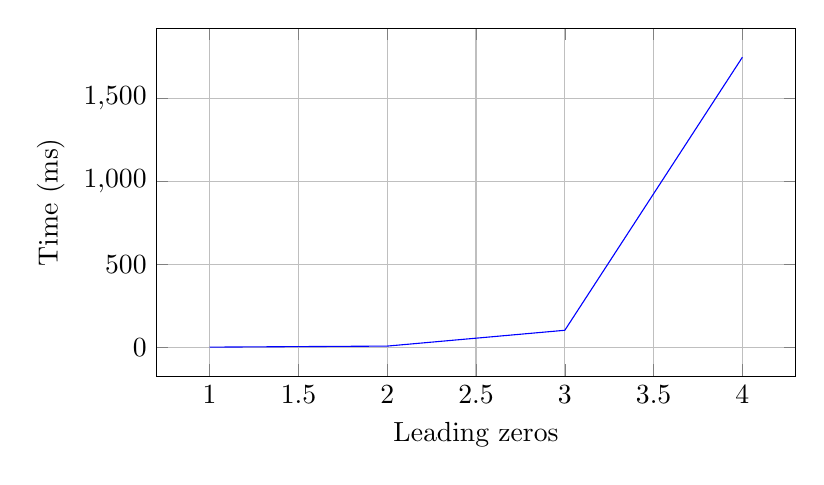
\begin{tikzpicture}
    \begin{axis}[
      xlabel={Leading zeros},
      ylabel={Time (ms)},
      grid=major,
      width=0.8\textwidth,
      height=6cm,
    ]
    \addplot[mark=., blue] coordinates {
      (1, 0.453130)
      (2, 6.818939)
      (3, 102.240562)
      (4, 1750.663366)
    };
    \end{axis}
  \end{tikzpicture}
  \caption[]{Time required to generate a Peer Id with a certain number of leading zeros.}
  \label{fig:pretty-graph}
\end{figure}

\section{Decentralized Verifier}
